\section{La programmation orientée objet sous CodeSys}


\begin{UPSTIidee}{Application : Etape d'un grafcet}
    Afin de faciliter la compréhension de cette partie, nous allons construire, tout au long de ce cours, une classe \emph{CStep} qui représente une étape d'un grafcet. Cette classe contiendra les attributs et méthodes suivants :

    \begin{minipage}{.45\linewidth}
        \paragraph{Attributs}
        \begin{itemize}
            \item \textbf{m\_xActivityBit} : bit d'activité (actif ou non)
                  \begin{itemize}
                      \item Accessible en lecture uniquement
                  \end{itemize}
            \item \textbf{m\_tActivationDuration} : Stocke le temps d'activation de l'étape
                  \begin{itemize}
                      \item Accessible en lecture uniquement
                  \end{itemize}
            \item \textbf{m\_tTaskPeriod} : période de la tâche
                  \begin{itemize}
                      \item Accessible en lecture et en écriture
                  \end{itemize}
        \end{itemize}
    \end{minipage}%
    \begin{minipage}{.45\linewidth}
        \paragraph{Méthodes}
        \begin{itemize}
            \item \textbf{MInit} : Méthode appelée à l'initialisation du programme
            \item \textbf{MActivate} : active l'étape
            \item \textbf{MDeactivate} : désactive l'étape
        \end{itemize}
    \end{minipage}

\end{UPSTIidee}

\subsection{Les classes}

On l'a vu, la notion de classe nous demande de pouvoir créer des attributs et des méthodes. Les attributs sont des variables internes aux classes qui devront être conservées entre deux utilisations d'un objet de cette classe.
L'utilisation de fonctions (POU FUNCTION) ne serait pas satisfaisante, car la durée de vie d'une variable interne à une fonction est limitée à l'exécution de cette fonction.

A l'inverse, un bloc fonctionnel s'utilise après en avoir créé une instance et ses variables internes sont conservées entre d'une utilisation à l'autre. Les POU FB semblent donc adaptées à la création de classes.

\UPSTIaRetenir{Nous utiliserons les blocs fonctions pour implémenter la notion de classe sous CodeSys.}

\begin{UPSTIinfor}{Déclaration d'une classe sous CodeSys}
    Définir une classe sous CodeSys revient à définir un bloc fonctionnel. Afin de différencier les variables privées (inaccessibles depuis l'extérieur) des attributs publics (accessibles depuis l'extérieur), on utilisera la convention suivante :
    \begin{itemize}
        \item Les variables publiques commenceront par \emph{m\_}
        \item les variables privées n'ont pas de préfixe particulier
    \end{itemize}

    Ainsi, la déclaration d'une classe \lstinline[language=ST]{<CName>} se fera de la manière suivante :
    \begin{lstlisting}
        FUNCTION_BLOCK <CName> (* définition de la classe <CName> *)
            VAR
                <type><Name> : <type>; (* variable locale non accessible de l'extérieur *)
                m_<type><Name> : <type>; (* membre de l'objet accessible de l'extérieur sous certaines conditions*)
            END_VAR
    \end{lstlisting}
\end{UPSTIinfor}

\begin{UPSTIidee}{}
    Puisqu'elle ne possède que des attributs accessibles, la déclaration de notre classe \emph{CStep} se fera de la manière suivante :
    \begin{lstlisting}
FUNCTION_BLOCK FB_CStep
    VAR
        m_xActivityBit : BOOL; (* bit d'activité (actif ou non) *)
        m_tActivationDuration : TIME; (* Stocke le temps d'activation de l'étape *)
        m_tTaskPeriod : TIME; 
    END_VAR\end{lstlisting}

    L'instanciation d'un objet de cette classe pourra alors s'écrire \lstinline{Etape1 : FB_CStep;}

    Pour le moment, ces attributs ont été déclarés dans notre classe \emph{CStep} mais ils ne sont pas accessibles depuis l'extérieur (Il est impossible d'évaluer l'expression \lstinline{Etape1.m_xActivityBit}). Ces variables sont "coincées" à l'intérieur de notre bloc fonction. Pour les rendre accessibles, nous allons utiliser l'objet \lstinline{PROPERTY} proposé par CodeSys. 
\end{UPSTIidee}

\subsection{L'objet PROPERTY (propriété)}
L'objet \lstinline{PROPERTY} est un outil proposé par CodeSys pour la programmation orientée objet. Il permet de définir des attributs (variables) propres à un contexte avec un niveau d'accessibilité paramétrable (publique, privée, protégée ou interne).

Cela signifie que l'on peut définir des variables à l'intérieur d'une classe qui pourront être accessibles depuis l'extérieur de la classe par l'intermédiaire de méthodes appelées \emph{accesseurs}.

\begin{UPSTIinfor}{Les accesseurs}
    Il existe deux types d'accesseurs : GET et SET. 
    \begin{description}
        \item[GET] : Permet de lire la valeur d'une variable
        \item[SET] : Permet d'écrire la valeur d'une variable
    \end{description}
\end{UPSTIinfor}

Une propriété est donc un objet que l'on associe à une POU. On décrit ensuite ses accesseurs pour définir comment lire ou écrire la valeur de la propriété.

\begin{UPSTIidee}{}
    
\end{UPSTIidee}




\subsection{Méthodes}
L'objet \lstinline{METHOD} est un outil proposé par CodeSys pour la programmation orientée objet. Il permet de définir des méthodes (fonctions) propres à un contexte avec un niveau d'accessibilité paramétrable (publique, privée, protégée ou interne).

Comme une fonction, on peut définir :
\begin{itemize}
    \item Des variables d'Entrées, de sorties ou d'entrées-sorties
    \item Des variables locales à la méthode
          \begin{itemize}
              \item La durée de vie de ces variables locales est alors limitée à l'exécution de la méthode
          \end{itemize}
\end{itemize}

Par ailleurs, \textbf{une méthode a accès au contexte de l'instance à laquelle elle est associée}. Cela signifie qu'elle a accès aux variables et méthodes de l'objet dont elle dépend.

Enfin, CodeSys autorise la déclaration de \lstinline{METHOD}s dans une interface. Elle devra alors être implémentée dans les classes qui implémentent cette interface.

\UPSTIaRetenir{Les méthodes des classes que nous définirons seront des méthodes associées au bloc fonction concerné.}

\begin{UPSTIidee}{Les méthodes de la classe CStep}
    Les méthodes de la classe \emph{CStep} seront définies dans le bloc fonctionnel \emph{FB\_CStep}. Elles seront donc des méthodes associées à ce bloc fonctionnel.

    \begin{minipage}[t]{.5\linewidth}
        \paragraph{Méthodes}
        \begin{itemize}
            \item \textbf{MInit} : Méthode appelée à l'initialisation du programme
            \item \textbf{MActivate} : active l'étape
            \item \textbf{MDeactivate} : désactive l'étape
        \end{itemize}
    \end{minipage}%
    \begin{minipage}[t]{.4\linewidth}
        \begin{lstlisting}
METHOD MInit : BOOL
    VAR_INPUT
    END_VAR
    VAR_OUTPUT
    END_VAR
    VAR
    END_VAR
    // Code de la méthode
    // ...
    // Fin du code de la méthode
END_METHOD
        \end{lstlisting}
    \end{minipage}
\end{UPSTIidee}

\begin{UPSTIinfor}{Ajout d'un propriété sous CodeSys}
    \begin{minipage}{.7\linewidth}
        Sous CodeSys, les propriétés et les méthodes sont ajoutés à la POU en utilisant l'outil \emph{Add Object}. Il suffit alors de sélectionner le type de l'objet à ajouter (propriété ou méthode) et de le nommer.
    \end{minipage}\hfill
    \begin{minipage}{.2\linewidth}
        \centering
        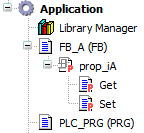
\includegraphics[width=\linewidth]{_cds_img_property.png}
    \end{minipage}    
\end{UPSTIinfor}

\subsection{Les interfaces}
Une interface est un ensemble de méthodes et de propriétés qui définissent un contrat. Une classe qui implémente une interface doit alors implémenter toutes les méthodes et propriétés de cette interface. Cela permet de définir une structure très générique qui sera utilisée, ensuite, par les classes que nous définirons. 

\UPSTIaRetenir{Les interfaces permettent de définir un contrat que les classes qui les implémentent doivent respecter. La déclaration d'une interface se fait de la même manière que la déclaration d'une classe, mais aucune méthode n'est implémentée.}
\lstDeleteShortInline~
\begin{UPSTIactivite}[][Exemple d'interface]
    \UPSTIquestion{Donner un exemple dans lequel l'utilisation d'une interface est pertinente, par exemple dans le monde du jeu vidéo. Expliquer}
    \vspace{5cm}
\end{UPSTIactivite}

\begin{UPSTIinfor}{Les interfaces sous CodeSys}
    \begin{minipage}{.7\linewidth}
        Sous CodeSys, une interface s'ajoute dans l'arborescence du projet en utilisant l'outil \emph{Add Object}. Il suffit alors de sélectionner le type de l'objet à ajouter (interface) et de le nommer. Elle apparaît alors ainsi que les méthodes et propriétés qui lui sont associées. 
        
        Le mot clef utilisé sous CodeSys est \lstinline{INTERFACE}.


        Le mot clef \lstinline{IMPLEMENT} est utilisé lors de la déclaration d'une classe pour indiquer que cette classe implémente une interface.
        
    \end{minipage}
    \hfill
    \begin{minipage}{.25\linewidth}
        \centering
        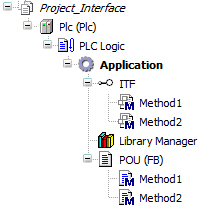
\includegraphics[width=\linewidth]{_cds_img_itf_method.png}
    \end{minipage}

\end{UPSTIinfor}

\subsection{Les pointeurs spéciaux}
CodeSys défini deux vecteurs spéciaux \lstinline{THIS} et \lstinline{SUPER}. Leur utilisation est réservée au contexte de la POO, dans le corps d'un bloc fonctionnel ou dans les méthodes associées.
\subsubsection{le pointeur THIS} 

Le pointeur \lstinline{THIS} est un pointeur spécial qui pointe vers l'objet auquel appartient la méthode. Il est automatiquement disponible dans tous les blocs fonctions. 

Les utilisations principales de \lstinline{THIS} sont données ci-dessous, les exemples sont extraits de la documentation en ligne de CodeSys. 

\paragraph{Démasquage d'une propriété ou d'une méthode : } Par exemple, lorsqu'une variable locale a le même nom qu'une propriété de l'objet, il est nécessaire de démasquer l'objet pour accéder à la propriété.  

\lstinputlisting[multicols=2]{this_exemple1.st}

\paragraph{Désigner l'objet tout entier} lors d'un passage d'objet en paramètre d'une méthode.

\lstinputlisting[multicols=2]{this_exemple2.st}

\subsubsection{Le pointeur SUPER}
Le pointeur \lstinline{SUPER} est un pointeur spécial qui pointe vers l'objet parent de l'objet auquel appartient la méthode. Il est automatiquement disponible dans tous les blocs fonctions. Par définition, son utilisation est réservée aux blocs fonctionnels obtenus par dérivation. 

Ce pointeur permet d'accéder aux méthodes et propriétés de l'objet parent, notamment quand celles-ci ont été surchargées dans les blocs fonctionnels dérivés. 

Le code suivant, issu de la documentation en ligne de CodeSys, montre quelques exemples d'utilisation des pointeurs \lstinline{SUPER} et \lstinline{THIS}.

\lstinputlisting[multicols=2]{super_exemple.st}

